% ============================================================================
%  Chapitre 4, partie II, 8. : Résultats de la simulation
%  Figures produites par scripts/run_case_a.py et scripts/run_case_iso.py
% ============================================================================

% ----------------------------------------------------------------------------
\subsection{Résultats de la simulation}

On applique l'algorithme à deux boules de même masse et de même rayon,
lancées de la même façon mais l'une anisotrope, l'autre isotrope.

\begin{hypotheses}[Paramètres communs]
    On considère une boule de paramètres suivants :
    \begin{itemize}
        \item $m = 1$ kg, $a = 0{,}1$ m, $g = 9{,}81$ m.s$^{-2}$,
        $\mu_s = 0{,}5$, soit $\mu_s\,m\,g \approx 4{,}9$ N.
        \item $r_0 = 0$, $\alpha_0 = (0{,}8;\ 0{,}7;\ 0)$ rad,
        $\vect{\Omega}_0 = (-0{,}31;\ 0{,}10;\ 5{,}30)$ rad.s$^{-1}$
        dans $\rep{s}$.
        \item $h = 10^{-3}$ s et $n = 5000$ pas, soit une durée de $5$ s.
    \end{itemize}
\end{hypotheses}

Les inerties $I_1, I_2, I_3$ ne peuvent pas être choisies librement :
elles doivent provenir d'une répartition de masse contenue dans la
boule.

\begin{proposition}[Inerties admissibles]
    Les moments principaux d'inertie
    $\mat{I}_b = \mathrm{diag}(I_1,I_2,I_3)$ d'une répartition de
    masse contenue dans la boule de centre $G$ et de rayon $a$
    vérifient
    \[
        I_i \leq I_j + I_k,
        \qquad \{i,j,k\} = \{1,2,3\}
    \]
    et
    \[
        I_1 + I_2 + I_3 \leq 2\,m\,a^2
    \]
\end{proposition}

\begin{demonstration}
    Sans perte de généralité, on se place dans le repère principal d'inertie, d'origine $G$ et
    d'axes $x$, $y$, $z$. Les moments principaux s'écrivent
    \[
        I_1 = \int (y^2 + z^2)\,\dd m,
        \qquad
        I_2 = \int (z^2 + x^2)\,\dd m,
        \qquad
        I_3 = \int (x^2 + y^2)\,\dd m
    \]
    On a donc
    \[
        I_1 + I_2 - I_3 = 2\int z^2\,\dd m \geq 0
    \]
    soit $I_3 \leq I_1 + I_2$, et de même pour les deux autres
    inégalités. Ensuite, en faisant la somme,
    \[
        I_1 + I_2 + I_3 = 2\int (x^2 + y^2 + z^2)\,\dd m
    \]
    Comme la masse est contenue dans la boule,
    $x^2 + y^2 + z^2 \leq a^2$, d'où
    \[
        I_1 + I_2 + I_3 \leq 2\,a^2\int \dd m = 2\,m\,a^2
    \]
\end{demonstration}
% ----------------------------------------------------------------------------
\subsubsection{Boule anisotrope}

On prend $\mat{I}_b = \mathrm{diag}(1{,}5;\ 8{,}5;\ 9{,}5)\cdot 10^{-3}$
kg.m$^2$. On a $I_3 \leq I_1 + I_2$ et
$\mathrm{tr}\,\mat{I}_b = 1{,}95\cdot 10^{-2} \leq 2\,m\,a^2$. On a donc une sphère anisotrope de configuration admissible. 

\begin{figure}[H]
    \centering
    \begin{subfigure}{0.42\textwidth}
        \centering
        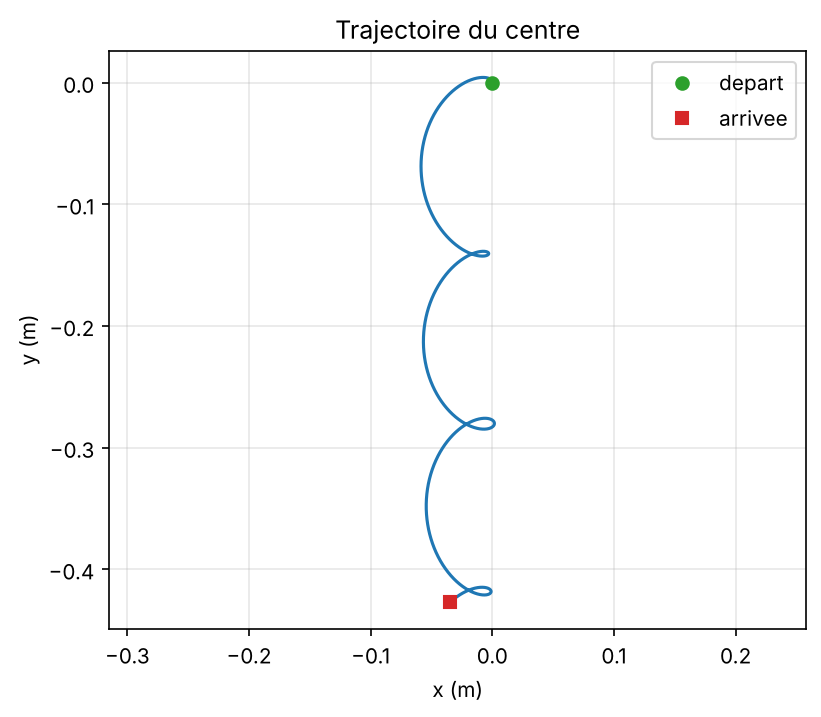
\includegraphics[width=\linewidth]{chapitre4/figures/case_a_trajectory.png}
        \caption{Trajectoire de $G$ dans le plan}
    \end{subfigure}
    \hfill
    \begin{subfigure}{0.52\textwidth}
        \centering
        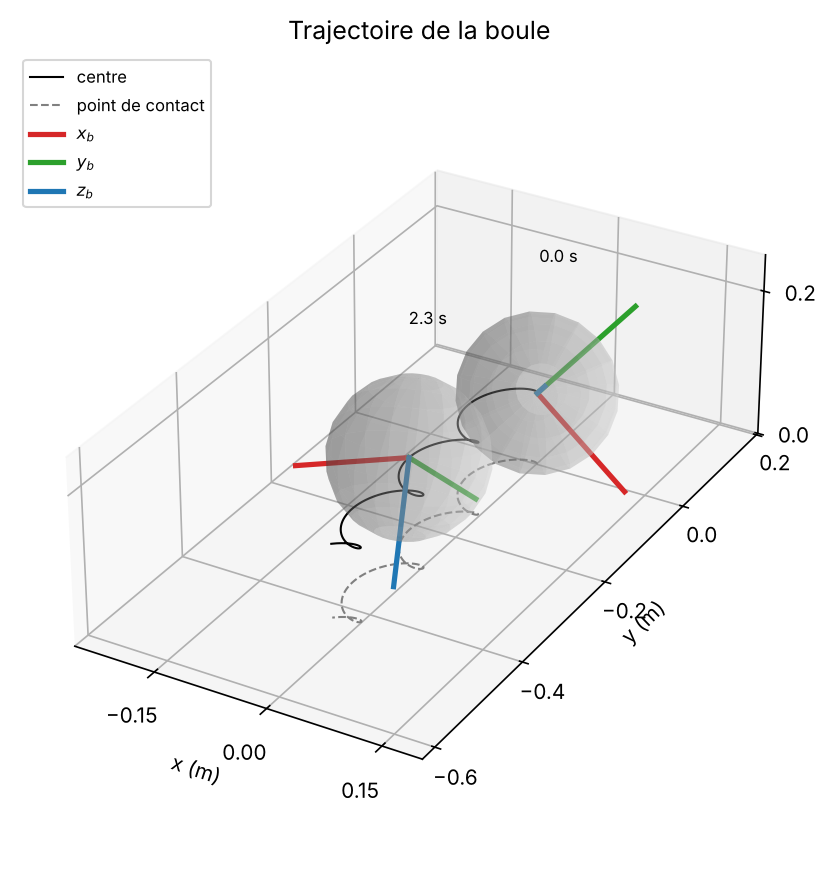
\includegraphics[width=\linewidth]{chapitre4/figures/case_a_trajectory_3d.png}
        \caption{Boule et axes du corps le long de la trajectoire}
    \end{subfigure}
    \caption{Boule anisotrope : trajectoire du centre $G$}
    \label{fig-traj-anisotrope}
\end{figure}

\begin{figure}[H]
    \centering
    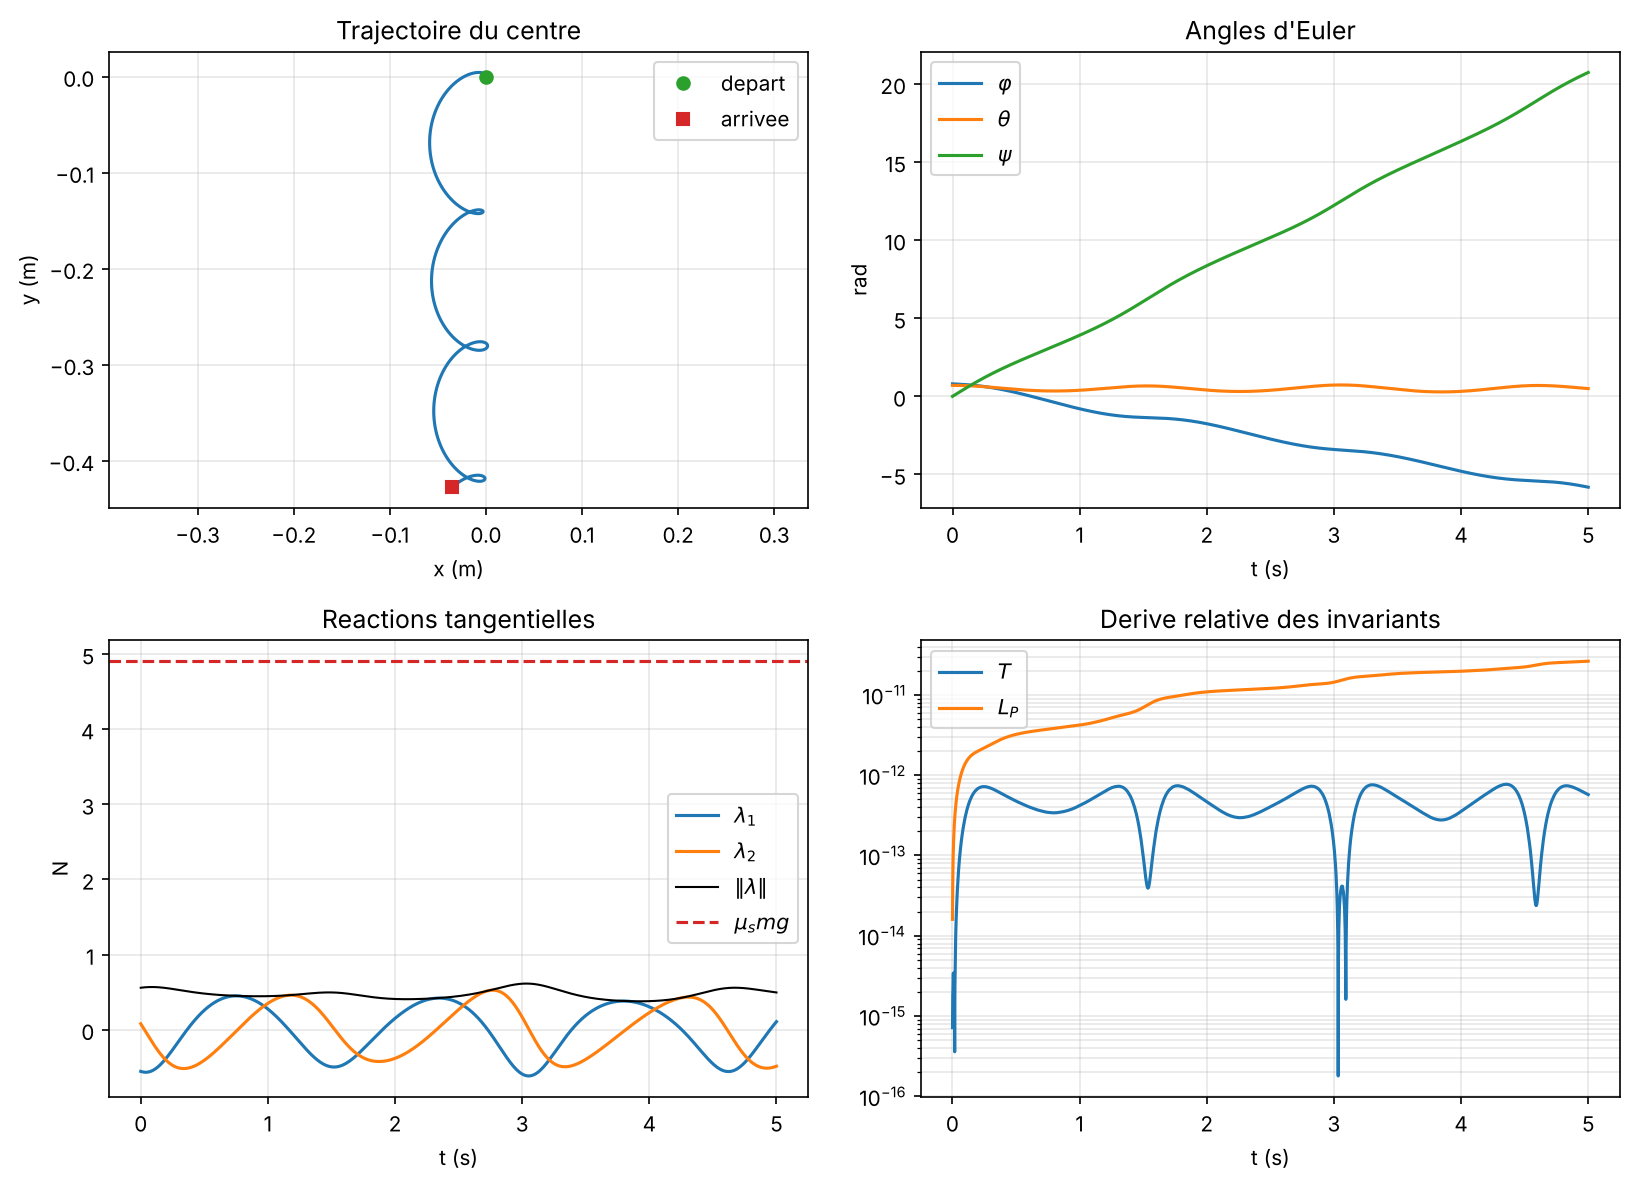
\includegraphics[width=0.9\textwidth]{chapitre4/figures/case_a_summary.png}
    \caption{Boule anisotrope : trajectoire, angles d'Euler, réactions
    tangentielles et dérive des invariants}
    \label{fig-resume-anisotrope}
\end{figure}

\textbf{Contrôles de la simulation :} Les hypothèses de validité sont vérifiées sur
toute la durée :
\begin{itemize}
    \item $|\cos\theta| \geq 0{,}75$ : les angles d'Euler restent loin
    de la singularité.
    \item $\|\vect{\lambda}_k\| \leq 0{,}62$ N $\ll \mu_s\,m\,g$ : pas de
    glissement, et $\mu_s \geq 0{,}07$ suffirait.
    \item Dérives relatives maximales : $8\cdot 10^{-13}$ pour $T$ et
    $3\cdot 10^{-11}$ pour $\vect{L}_P$.
\end{itemize}

% ----------------------------------------------------------------------------
\subsubsection{Boule isotrope}

On prend la boule homogène, $\mat{I}_b = \tfrac25\,m\,a^2\,\Id
= 4\cdot 10^{-3}\,\Id$ kg.m$^2$, avec le même lancer. C'est une sphère dont on connaît a priori la trajectoire, on l'utilise ici juste pour montrer la validité de la simulation.

\begin{proposition}[Boule isotrope]
    Si $\mat{I}_b = I_0\,\Id$, les frottements sont nuls,
    $\vect{\Omega}(t) = \vect{\Omega}_0$, et le centre suit un
    mouvement rectiligne uniforme
    \[
        r(t) = r_0 + a\,t\begin{pmatrix}
            \Omega_{0,y}\\ -\,\Omega_{0,x}
        \end{pmatrix}
    \]
\end{proposition}

\begin{demonstration}
    On note $\vect{F} = N_x\,\vect{e}_x + N_y\,\vect{e}_y$ le
    frottement en $P$. La vitesse du centre de masse s'écrit : 
    \[
        \vect{v}_G = a\,\vect{\Omega}\wedge\vect{e}_z
    \]
    La loi de Newton (ou le théorème de la quantité de mouvement) donne
    \[
        m\,\dot{\vect{v}}_G = \vect{F}
    \]
    Comme $\mat{I}_b = I_0\,\Id$, le moment cinétique en $G$ est
    $\vect{L}_G = I_0\,\vect{\Omega}$. Avec
    $\vect{GP} = -\,a\,\vect{e}_z$, le théorème du moment cinétique
    en $G$ donne
    \[
        I_0\,\dot{\vect{\Omega}}
        = -\,a\,\vect{e}_z\wedge\bigl(\vect{F} + N_z\,\vect{e}_z\bigr)
        = -\,a\,\vect{e}_z\wedge\vect{F}
    \]
    Or, on a : 
    \[
        \dot{\vect{v}}_G = a\,\dot{\vect{\Omega}}\wedge\vect{e}_z
        = -\,\frac{a^2}{I_0}\,(\vect{e}_z\wedge\vect{F})\wedge\vect{e}_z
    \]
    Comme $\vect{F}$ est horizontal,
    $(\vect{e}_z\wedge\vect{F})\wedge\vect{e}_z = \vect{F}$, donc
    \[
        \dot{\vect{v}}_G = -\,\frac{a^2}{I_0}\,\vect{F}
    \]
    En reinjectant dans la loi de Newton, on a :
    \[
        \Bigl(1 + \frac{m\,a^2}{I_0}\Bigr)\vect{F} = \vect{0} \longleftrightarrow \vect{F} = \vect{0}
    \]
    d'où $\vect{F} = \vect{0}$. On en déduit
    $\dot{\vect{\Omega}} = \vect{0}$ et $\dot{\vect{v}}_G = \vect{0}$,
    donc $\vect{v}_G = a\,\vect{\Omega}_0\wedge\vect{e}_z
    = a\,(\Omega_{0,y},\,-\,\Omega_{0,x},\,0)$.
\end{demonstration}

\begin{figure}[H]
    \centering
    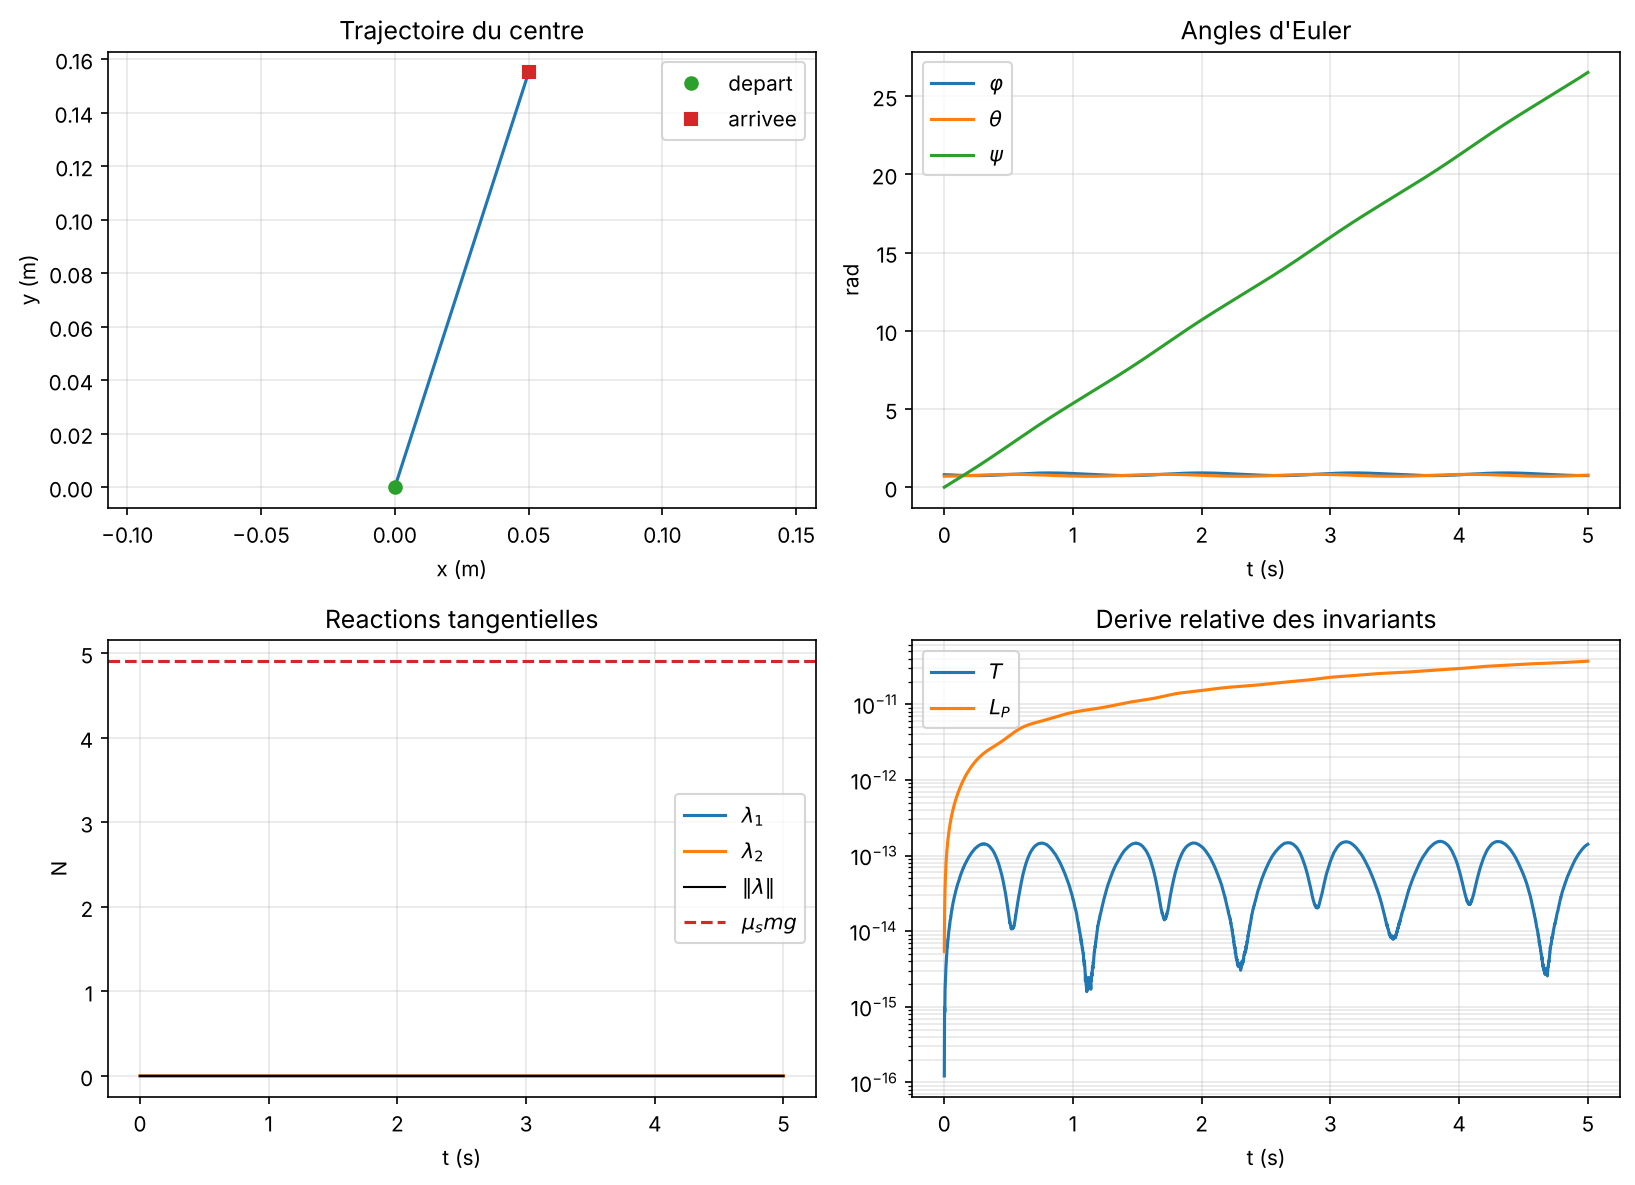
\includegraphics[width=0.9\textwidth]{chapitre4/figures/case_iso_summary.png}
    \caption{Boule isotrope : trajectoire, angles d'Euler, réactions
    tangentielles et dérive des invariants}
    \label{fig-resume-isotrope}
\end{figure}

La simulation retrouve cette solution avec (\cref{fig-resume-isotrope}) :
\[
    \max_k \|\vect{\Omega}_k - \vect{\Omega}_0\| \approx 6\cdot 10^{-11},
    \qquad
    \max_k \|r_k - r(t_k)\| \approx 1{,}5\cdot 10^{-11}\ \text{m},
    \qquad
    \max_k \|\vect{\lambda}_k\| \approx 10^{-16}\ \text{N}
\]
